\documentclass[conference]{IEEEtran}
\IEEEoverridecommandlockouts
% The preceding line is only needed to identify funding in the first footnote. If that is unneeded, please comment it out.
\usepackage{cite}
\usepackage{amsmath,amssymb,amsfonts}
\usepackage{algorithmic}
\usepackage{graphicx}
\usepackage{textcomp}
\usepackage{xcolor}
\usepackage{placeins}
\usepackage[hidelinks]{hyperref}
\usepackage{float}
\usepackage{subcaption}
\def\BibTeX{{\rm B\kern-.05em{\sc i\kern-.025em b}\kern-.08em
    T\kern-.1667em\lower.7ex\hbox{E}\kern-.125emX}}
\begin{document}

\title{Redes Neurais Convolucionais}

\author{\IEEEauthorblockN{Arthur Abrahão Santos Barbosa}
\IEEEauthorblockA{\textit{Universidade Federal de Pernambuco} \\
\textit{Centro de Informática}\\
Pernambuco, Brasil \\
aasb2@cin.ufpe.br}
\and
\IEEEauthorblockN{Arthur Henrique}
\IEEEauthorblockA{\textit{Universidade Federal de Pernambuco} \\
\textit{Centro de Informática}\\
Pernambuco, Brasil \\
ahac@cin.ufpe.br}
\and
\IEEEauthorblockN{Filipe Samuel da Silva}
\IEEEauthorblockA{\textit{Universidade Federal de Pernambuco} \\
\textit{Centro de Informática}\\
Pernambuco, Brasil \\
fss8@cin.ufpe.br}
\and
\IEEEauthorblockN{Vinicius Bastos Moreira Principe}
\IEEEauthorblockA{\textit{Universidade Federal de Pernambuco} \\
\textit{Centro de Informática}\\
Pernambuco, Brasil \\
vbmp@cin.ufpe.br}
}

\maketitle



% \begin{abstract}
%     This document is a model and instructions for \LaTeX.
%     This and the IEEEtran.cls file define the components of your paper [title, text, heads, etc.]. *CRITICAL: Do Not Use Symbols, Special Characters, Footnotes, 
%     or Math in Paper Title or Abstract.
%     \end{abstract}
    
% \begin{IEEEkeywords}
% component, formatting, style, styling, insert
% \end{IEEEkeywords}




\section{Introduction}




\section{Database}

A base de dados usada veio da junção das bases de dados de acidentes de carro do condado de Montgomery 
\cite{incidents} e da base de informação dos motoristas involvidos nestes acidentes \cite{drivers}

\subsection{Scope and Data selection}
\subsection{Target definition}
\subsection{Pre-processing Data}

\section{Extraction of knowledge, results and discussion}

\subsection{Logistic Regression}

\subsection{Decision Trees}

\subsection{Classification rules induction}
\subsection{Propensity score performance score}


\section{Conclusions}



% \begin{figure}[H]
% \centerline{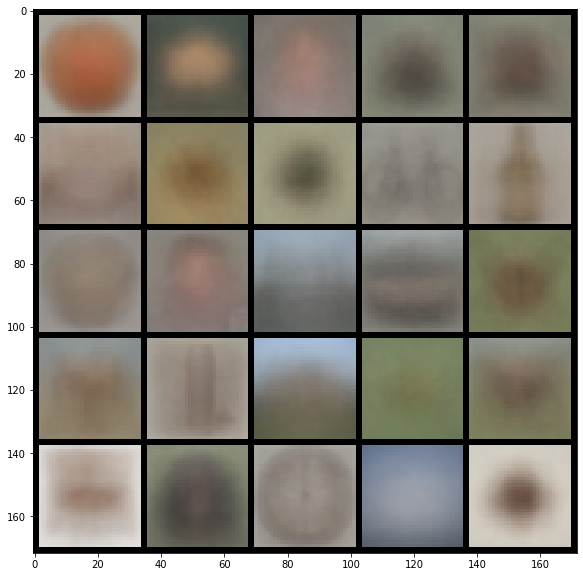
\includegraphics[width=0.4\textwidth]{Images/img_mean1.png}}
% \caption{\label{fig:img_mean1}Da esquerda para a direita, de cima para a baixo: apple, aquarium\_fish, baby, bear, beaver, bed, bee, beetle, bicycle, bottle, bowl, boy, bridge, bus, butterfly, camel, can, castle, caterpillar, cattle, chair, chimpanzee, clock, cloud, cockroach}
% \end{figure}

% \begin{figure}[H]
% \centerline{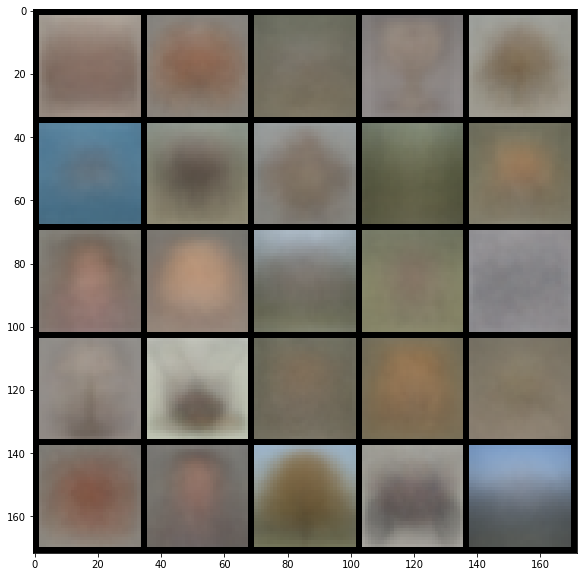
\includegraphics[width=0.4\textwidth]{Images/img_mean2.png}}
% \caption{\label{fig:img_mean2}Da esquerda para a direita, de cima para a baixo: couch, crab, crocodile, cup, dinosaur, dolphin, elephant, flatfish, forest, fox, girl, hamster, house, kangaroo, keyboard, lamp, lawn\_mower, leopard, lion, lizard, lobster, man, maple\_tree, motorcycle, mountain}
% \end{figure}

% \begin{figure}[H]
% \centerline{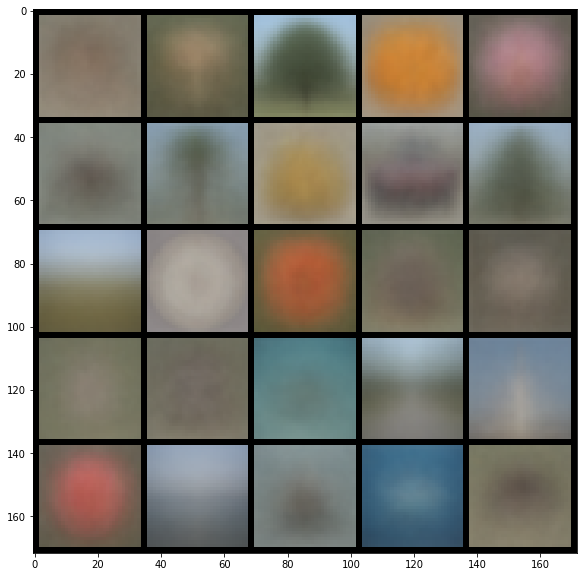
\includegraphics[width=0.4\textwidth]{Images/img_mean3.png}}
% \caption{\label{fig:img_mean3}Da esquerda para a direita, de cima para a baixo: mouse, mushroom, oak\_tree, orange, orchid, otter, palm\_tree, pear, pickup\_truck, pine\_tree, plain, plate, poppy, porcupine, possum, rabbit, raccoon, ray, road, rocket, rose, sea, seal, shark, shrew}
% \end{figure}

% \begin{figure}[H]
% \centerline{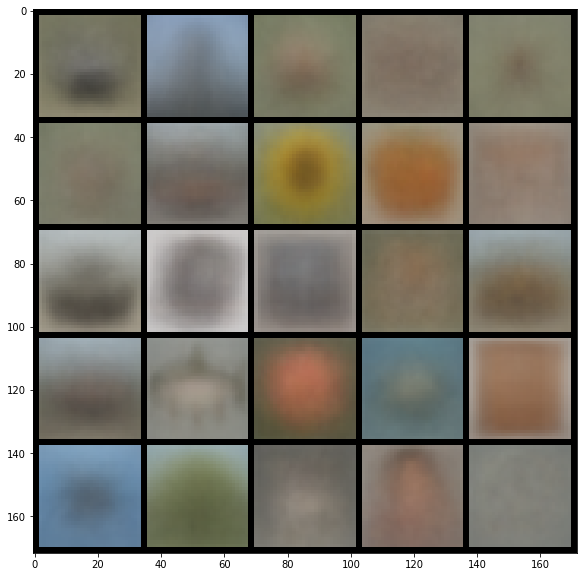
\includegraphics[width=0.4\textwidth]{Images/img_mean4.png}}
% \caption{\label{fig:img_mean4}Da esquerda para a direita, de cima para a baixo: skunk, skyscraper, snail, snake, spider, squirrel, streetcar, sunflower, sweet\_pepper, table, tank, telephone, television, tiger, tractor, train, trout, tulip, turtle, wardrobe, whale, willow\_tree, wolf, woman, worm}
% \end{figure}

% \begin{itemize}
% \item Média da Imagens Normalizadas
% \end{itemize}

% \begin{figure}[H]
% \centerline{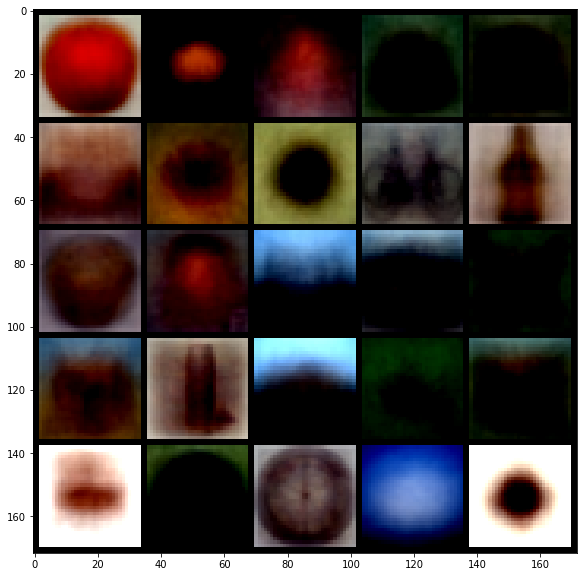
\includegraphics[width=0.4\textwidth]{Images/img_mean_norm1.png}}
% \caption{\label{fig:img_mean_norm1}Da esquerda para a direita, de cima para a baixo: apple, aquarium\_fish, baby, bear, beaver, bed, bee, beetle, bicycle, bottle, bowl, boy, bridge, bus, butterfly, camel, can, castle, caterpillar, cattle, chair, chimpanzee, clock, cloud, cockroach}
% \end{figure}

% \begin{figure}[H]
% \centerline{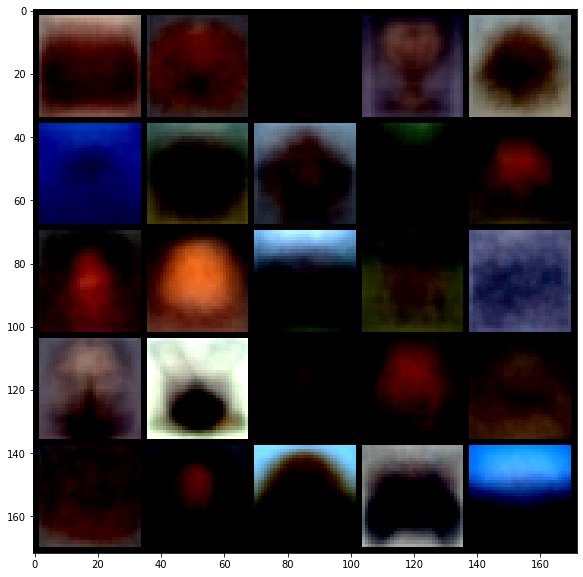
\includegraphics[width=0.4\textwidth]{Images/img_mean_norm2.png}}
% \caption{\label{fig:img_mean_norm2}Da esquerda para a direita, de cima para a baixo: couch, crab, crocodile, cup, dinosaur, dolphin, elephant, flatfish, forest, fox, girl, hamster, house, kangaroo, keyboard, lamp, lawn\_mower, leopard, lion, lizard, lobster, man, maple\_tree, motorcycle, mountain}
% \end{figure}

% \begin{figure}[H]
% \centerline{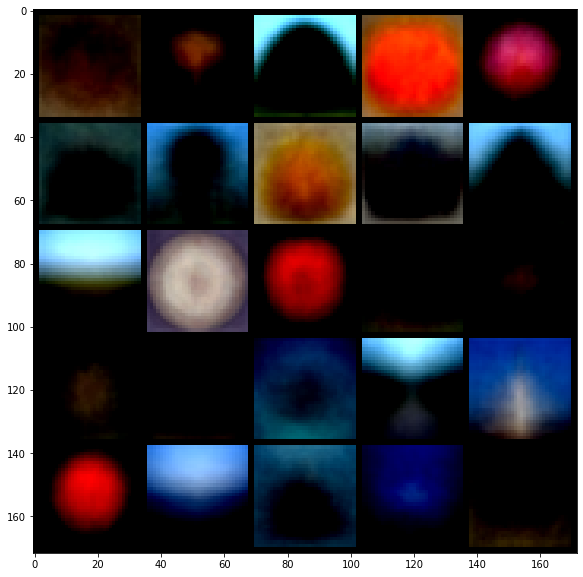
\includegraphics[width=0.4\textwidth]{Images/img_mean_norm3.png}}
% \caption{\label{fig:img_mean_norm3}Da esquerda para a direita, de cima para a baixo: mouse, mushroom, oak\_tree, orange, orchid, otter, palm\_tree, pear, pickup\_truck, pine\_tree, plain, plate, poppy, porcupine, possum, rabbit, raccoon, ray, road, rocket, rose, sea, seal, shark, shrew}
% \end{figure}

% \begin{figure}[H]
% \centerline{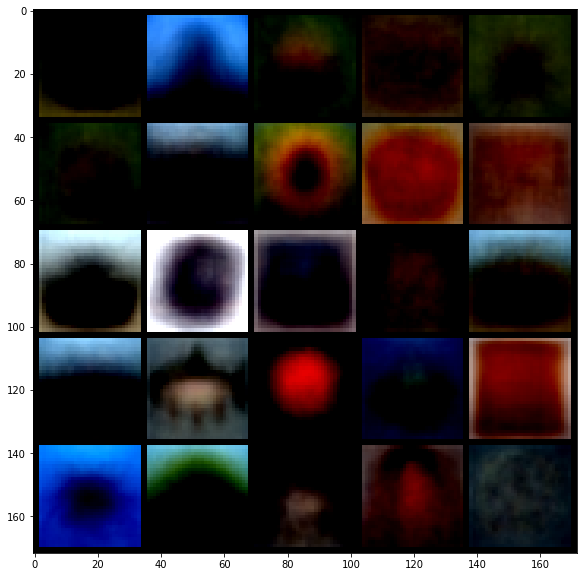
\includegraphics[width=0.4\textwidth]{Images/img_mean_norm4.png}}
% \caption{\label{fig:img_mean_norm4}Da esquerda para a direita, de cima para a baixo: skunk, skyscraper, snail, snake, spider, squirrel, streetcar, sunflower, sweet\_pepper, table, tank, telephone, television, tiger, tractor, train, trout, tulip, turtle, wardrobe, whale, willow\_tree, wolf, woman, worm}
% \end{figure}
    
%\subsection{Sobre o Projeto}
%Para montar o classificador foi necessário passar  pelas seguintes etapas:



% \section{Sobre as Métricas Utilizadas}

% \subsection{Precision}

% Precision é a razão
%     \begin{equation}
%         \frac{A_c}{A_c + A_e}
%     \end{equation}

%     onde:

%     \begin{itemize}
%     \item $A_c$ é o número de amostras corretamente classificadas de uma determinada classe.
%     \item $A_e$ é o número de amostras  erroneamente classificadas como sendo desta determinada classe.
%     \end{itemize}

%     Precision é intuitivamente a habilidade do classificador não marcar como pertencente a uma classe uma amostra que não pertence a esta. O melhor valor de Precision é 1 e o pior é zero.
%     \cite{b7}
% \subsection{Accuracy} 

% Accuracy é a fração de amostras preditas corretamente, e é dada pela seguinte fórmula:

% \begin{equation}
%     \frac{\sum\limits_{1}^{n}A_c}{\sum\limits_{1}^{n}A_t}
% \end{equation}







\bibliography{mybib}
\nocite{*}
\bibliographystyle{IEEEtran}
\end{document}
